Рассмотрим параллельную реализацию алгоритма поиска простых чисел.

\section{Описание алгоритма}
Пусть максимальное число поиска = $N$, а число потоков = $T$. Стандандартный алгоритм произведёт перебор чисел от 2 до $N$, проверяя каждое число на простоту. В случае, если проверка пройдена, число добавляется массив простых чисел. Параллельная версия отличается тем, что для i-го потока выделяются числа от 2+i до $N$ с шагом $T$.

Схема алгоритма приведена на рисунке 2.1, 2.2
\begin{figure}[h]
	\begin{center}
		{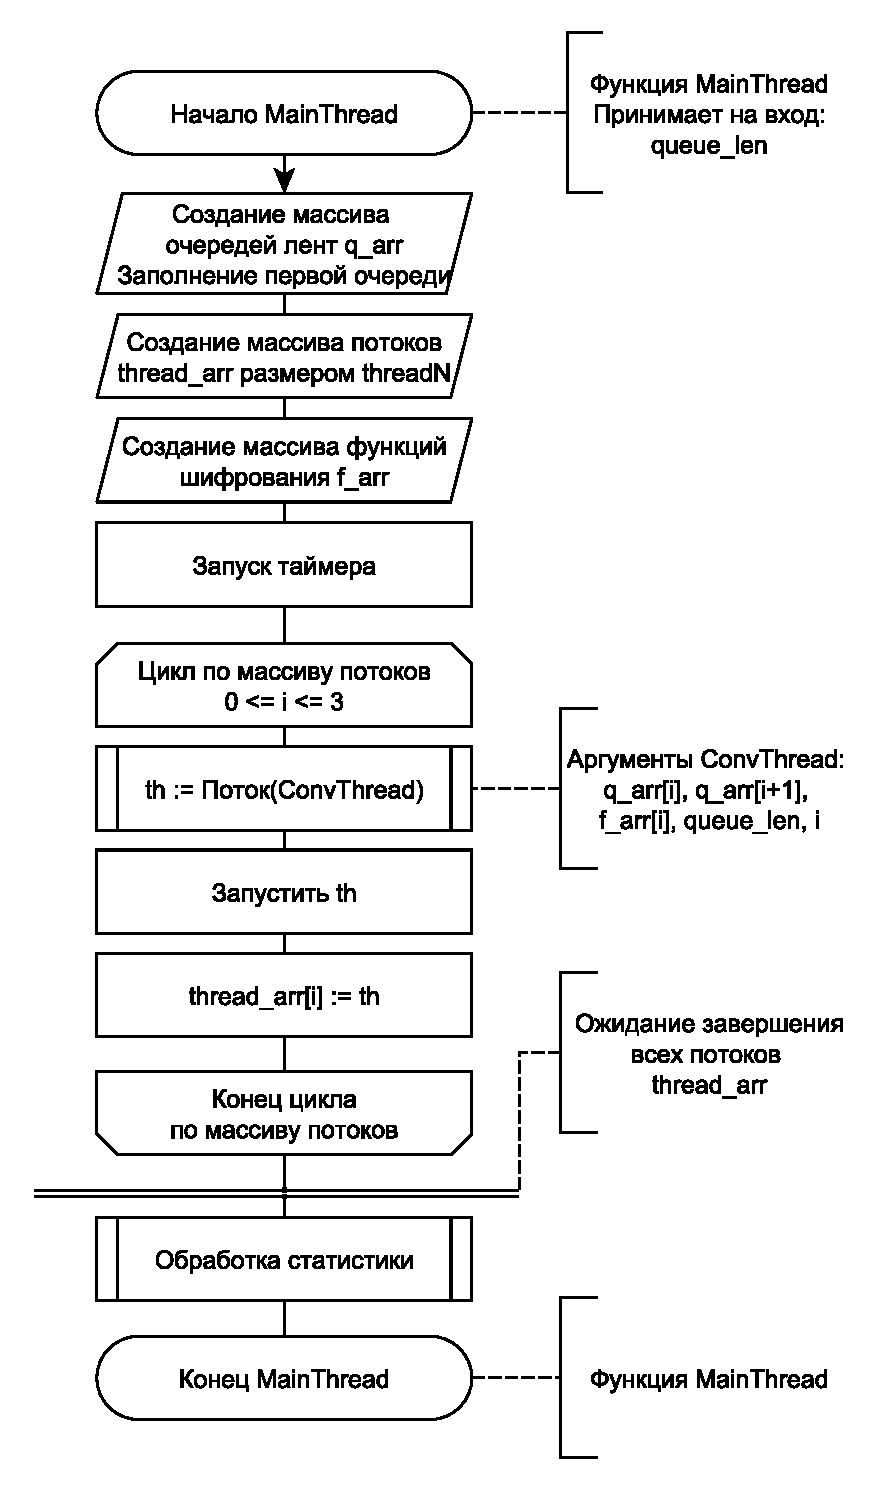
\includegraphics[height=20cm, width = 17cm]{Main}}
		\caption{Главный поток}
	\end{center}
\end{figure}
\begin{figure}[h]
	\begin{center}
		{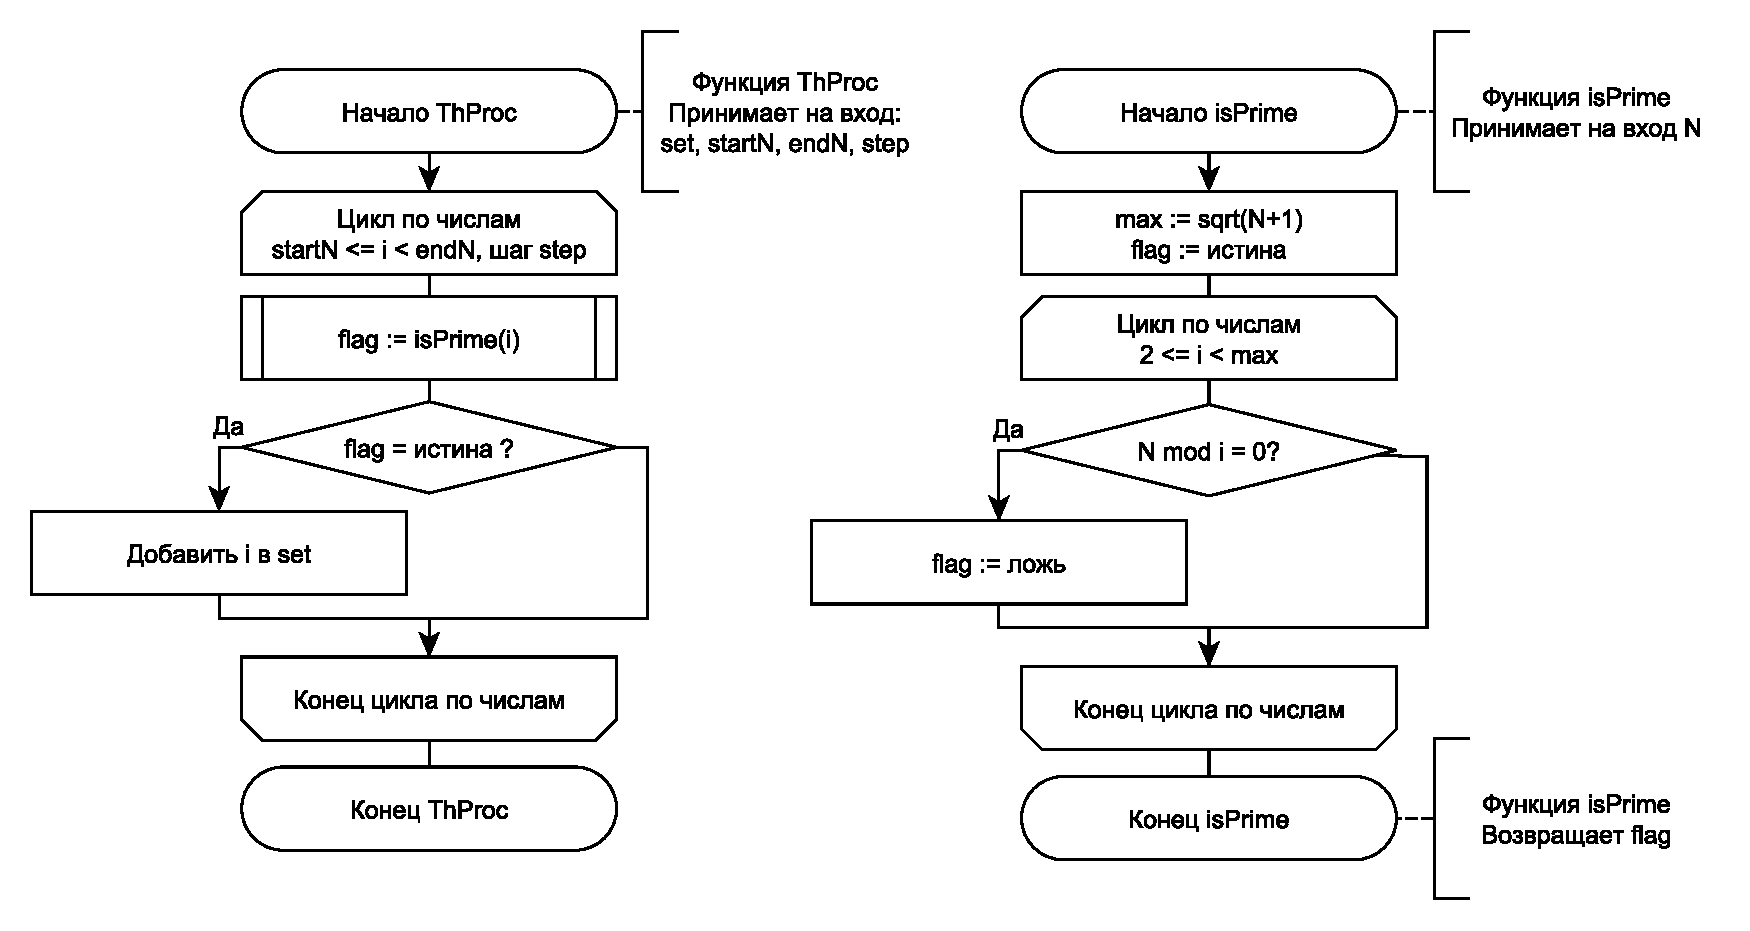
\includegraphics[height=15cm, width = 17cm]{Work}}
		\caption{Рабочий поток}
	\end{center}
\end{figure}



\section{Требования к программному обеспечению}
Для полноценной проверки и оценки алгоритмов необходимо выполнить следующее.
\begin{enumerate}
	\item Обеспечить возможность консольного ввода предела поиска и количества используемых потоков. Программа должна вывести множество простых чисел.
	\item Реализовать функцию замера процессорного времени, затраченного функцией.
\end{enumerate}


\section{Заготовки тестов}
При проверке алгоритма необходимо будет использовать следующие классы тестов:
\begin{itemize}
	\item один поток, несколько потоков;
	\item предел = 2, предел = произвольное число;
\end{itemize}

\section*{Вывод}
Результатом конструторской части стало схематическое описание параллельного алгоритма нахождения простого числа, сформулированны тесты и требования к программному обеспечению.



